
 \subsection{Regressão logística}
%  chrome-extension://efaidnbmnnnibpcajpcglclefindmkaj/https://bdm.unb.br/bitstream/10483/34269/1/2022_JessicaArrudaArcanjo_tcc.pdf
 A regressão logística é um método estatístico utilizado para modelar a probabilidade condicional de uma variável,
 dado um conjunto de covariáveis. É comumente utilizada para problemas de classificação binária, onde a variável
dependente possui apenas duas categorias, como sim/não, positivo/negativo, 0/1 \cite{hosmer}.


O modelo de regressão logística é construído considerando a probabilidade da variável aleatória $Y$ ser igual a 1, onde Y é 
uma variável aleatória com distribuição Bernoulli, com probabilidade p de sucesso, cuja fórmula é dada por:

\begin{equation}
  P(Y=1| x_1, x_2, ..., x_k) = \frac{1}{1 + e^{-(\beta_0 + x_{1}\beta_1 + x_{2}\beta_2 + \ldots + x_{k}\beta_k)}},
  \label{eq:model_logistic}
\end{equation}

\noindent onde cada variável explicativa $(x_1, x_2, ..., x_k)$ tem um parâmetro $\beta$ correspondente, influenciando o resultado de $Y$.

A estimação dos parâmetros $(b_0, b_1, b_2, ..., b_k)$  na regressão logística é geralmente realizada por meio 
do método da máxima verossimilhança. O objetivo é encontrar os valores dos coeficientes que maximizam a função de
verossimilhança, representando a probabilidade de observar os dados observados dado o modelo.
 
A função de verossimilhança $L(\beta)$ para a regressão logística é dada pelo produto das probabilidades condicionais
de observar os eventos (valores da variável dependente) dados os valores das variáveis independentes. Para facilitar o cálculo, 
geralmente trabalhamos com o logaritmo natural da função de verossimilhança, conhecido como log-verossimilhança $l(\beta)$.

A log-verossimilhança para a regressão logística é:

\begin{equation}
  l(\beta) = \sum_{i=1}^{N} [y_i \beta^T x_i - \log(1 + e^{\beta^T x_i})], 
\end{equation}

\noindent onde,
\begin{itemize}
  \item  $N$é o número total de observações;
  \item  $y_i$ é a variável dependente binária da i-ésima observação (0 ou 1);
  \item $x_i$ é o vetor de covariáveis da $i$-ésima observação;
  \item \textbf{$\beta$} é o vetor de parâmetros do modelo modelo logístico.
\end{itemize}

A ideia é encontrar os valores de $(b_0, b_1, b_2, ..., b_k)$ que maximizam essa função. Isso geralmente é feito usando métodos computacionais, 
como o algoritmo de otimização Newton-Raphson ou o Gradiente Descendente \cite{curry1944}.

\subsubsection{Interpretação}

% definição de chance

Para a interpretação do modelo logístico é utilizada a Razão de Chances, que calcula a razão entre duas chances, sendo a chance 
(ou, do inglês, \textit{odds})
de um evento definida como a probabilidade do sucesso do evento sobre a probabilidade do fracasso \cite{szumilas2010explaining}.

\begin{equation}
  \text{Chance} =  \frac{P(Y=1|X=x)}{P(Y=0|X=x)}.
\end{equation}

Para calcular a Razão de Chances, inicialmente, é determinada a chance de ocorrência de um
$Y$ dado um conjunto de covariáveis x
Em seguida, é calculada a chance desse mesmo evento ocorrer quando, por exemplo,
a k-ésima covariável 
correspondente é incrementada em uma unidade. 
Dessa forma, a fórmula para a Razão de Chances (RC) é expressa por:

\begin{equation}
  \text{Razão de Chances} =  \frac{\frac{P(Y=1 | X` \text{ e } X_j = x_j + 1)}{P(Y=0 | X` \text{ e } X_j = x_j + 1)}}{\frac{P(Y=1 | X` \text{ e } X_j = x_j)}{P(Y=0 | X` \text{ e } X_j = x_j)}}, 
\end{equation}

\noindent onde, $X`$ é um vetor com todas as covariáveis exceto a covariável $X_j$.

Considerando a Equação \ref{eq:model_logistic}, temos que a Razão de Chances pode ser calculada como:

\begin{equation}
  RC = \exp{(\beta_j)}.
\end{equation}

Logo, para o crescimento de 1 unidade em $X_k$, variável associada ao $\beta_j$, a chance do evento ocorrer 
é multiplicada por $\exp{(\beta_j)}$ unidades, considerando as demais variáveis constantes. 
Ou seja, uma RC igual a 1 indica que a variável independente não tem efeito no resultado de $Y$ (nenhuma associação).
Uma RC maior que 1 sugere uma associação positiva, enquanto uma RC menor que 1 sugere uma associação negativa.

Outra medida interpretativa é a função log odds ou logíto. Ela é uma função que calcula o log da chance, ou seja, o 
log da razão das probabilidades do evento acontecer e dele não acontecer, cuja formulação é dada por:

\begin{equation}
  \text{logit}(P(Y=1)) = \log \left( \frac{P(Y=1)}{1 - P(Y=1)} \right),
\end{equation}

\noindent onde esse resultado nada mais é do que o preditor linear $\beta_0 + X_{1}\beta_1 + X_{2}\beta_2 + \ldots +X_{k}\beta_k$. 

Portanto, um coeficiente $\beta_j$ positivo indica que o aumento na respectiva covariável está associado a um aumento na log-odds 
(e, portanto, na probabilidade de sucesso), enquanto um coeficiente negativo está associado a uma diminuição nas log-odds (e na probabilidade de
sucesso).


\subsection{Redes neurais artificiais}

Redes Neurais Artificiais (ou \textit{Deep Learning}) é uma técnica de modelagem de dados
 presente no campo de Inteligência Artificial. As redes neurais tem sido amplamente utilizadas devido ao seu alto
  poder preditivo e também à flexibilidade de se aplicar esse método em diversos contextos, permitindo
   ser um modelo com menos restrições que os modelos tradicionais estatísticos \cite{mitnews_neuralnetworks}.


\subsubsection{Neurônio}

Uma rede neural tem esse nome devido à tentativa de se reproduzir o comportamento do cérebro humano.
 Sua arquitetura é composta por um conjunto de unidades denominadas neurônios, e cada neurônio é 
 responsável por receber informações, fazer o tratamento do que foi recebido, e repassar o resultado 
 para frente \cite{ai_3rd_edition}. A Figura \ref{fig:neuronio} ilustra a estrutura de 1 neurônio.
  Quando as informações $x_i$ entram no neurônio, acontece primeiramente um processo 
  onde é ponderada cada informação que foi recebida, pelos chamados \textbf{pesos}. Logo
   em seguida ocorre a soma dessa combinação linear. Feito isso, é realizado mais um processo 
   de soma, agora adicionando uma informação própria daquele neurônio nesse resultado. 
   Essa informação é chamada de \textbf{bias} (ou Viés). Antes desse resultado ser repassado 
   para outro neurônio, ele passa por uma função que vai definir a natureza daquela informação, 
   chamada de \textbf{função de ativação}, retornando assim uma saída $y$.
 \begin{figure}[H]
    \centering
     \caption{Neurônio da Rede neural}
    \begin{tikzpicture}[
init/.style={
  draw,
  circle,
  inner sep=2pt,
  font=\Huge,
  join = by -latex
},
squa/.style={
  draw,
  inner sep=2pt,
  font=\Large,
  join = by -latex
},
start chain=2,node distance=13mm,
scale = 0.6
]
\node[on chain=2] 
  (x2) {$x_2$};
\node[on chain=2,join=by o-latex] 
  {$w_2$};
\node[on chain=2,init] (sigma) 
  {$\displaystyle\Sigma$};
\node[on chain=2,squa,label=above:{\parbox{2cm}{\centering Função de Ativação}}]   
  {$f$};
\node[on chain=2,label=above:Saída,join=by -latex] 
  {$y$};
\begin{scope}[start chain=1]
\node[on chain=1] at (0,1.5cm) 
  (x1) {$x_1$};
\node[on chain=1,join=by o-latex] 
  (w1) {$w_1$};
\end{scope}
\begin{scope}[start chain=3]
\node[on chain=3] at (0,-1.5cm) 
  (x3) {$x_3$};
\node[on chain=3,label=below:Pesos,join=by o-latex] 
  (w3) {$w_3$};
\end{scope}
\node[label=above:\parbox{2cm}{\centering Viés \\ $b$}] at (sigma|-w1) (b) {};

\draw[-latex] (w1) -- (sigma);
\draw[-latex] (w3) -- (sigma);
\draw[o-latex] (b) -- (sigma);

\draw[decorate,decoration={brace,mirror}] (x1.north west) -- node[left=10pt] {Entradas} (x3.south west);
\end{tikzpicture}
   
    \label{fig:neuronio}
\end{figure} 

A Figura \ref{fig:neuronio} pode ser representada matematicamente da seguinte maneira:
\begin{equation}
    y = f (\beta + \sum_{i=1}^{d_x} w_ix_{i} ) ,
    \label{neuronio}
\end{equation}
 
\noindent onde, $d_x$ é o número de entradas.


\begin{figure}[H]
    \centering
    \caption{Tipos de Função de Ativação.}
    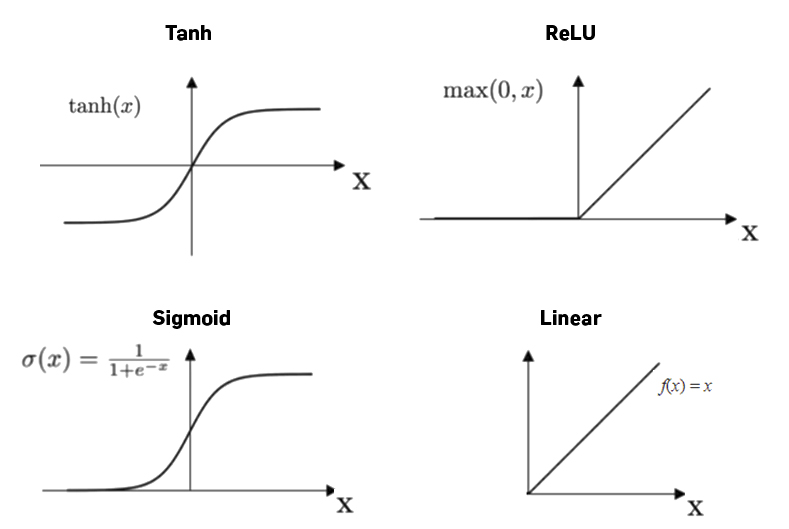
\includegraphics[scale=0.4]{imagens/activation-functions3.jpg}
    \caption*{Fonte: https://machine-learning.paperspace.com/wiki/activation-function}
    \label{fig:func_ativac}
    
\end{figure}

A Figura \ref{fig:func_ativac} mostra alguns tipos de funções de ativação que um neurônio pode ser utilizado.
Note como a maioria dessas funções restringe o valor de sua entrada. No caso 
da função Sigmoide e da Tangente hiperbólica (tanh), o valor da saída é limitado em um intervalo. Já a ReLU,
 desconsidera os valores negativos, e por fim existe a função Linear que apenas repassa a mesma informação para
 frente.

\vspace{1cm}

\subsubsection{Arquitetura}

Uma rede neural é estruturada em camadas formadas por um conjunto de neurônios. Conforme ilustrado
 na Figura \ref{fig:arc_smp_rnp}, temos as camadas de entrada, as camadas ocultas e a camada de saída. 
 A camada de entrada é o ponto de partida da rede neural, pois é onde as informações das variáveis entram. 
 Logo em seguida encontram-se as camadas ocultas, que são as principais responsáveis por criar redes mais complexas,
  pois o número de camadas e o número de neurônios dentro dessas camadas podem ser moldados ou adicionados dependendo 
  do objetivo empregado pela rede, conforme ilustrado na Figura \ref{fig:arc_cpx_rnp}. E por fim existe a camada de 
  saída, contendo o(s) valor(es) predito(s) pela rede \cite{zell_1994}.

\begin{figure}[H]
\centering
\caption{Rede Neural com uma camada oculta}
\begin{tikzpicture}[
plain/.style={
  draw=none,
  fill=none,
  },
net/.style={
  matrix of nodes,
  nodes={
    draw,
    circle,
    inner sep=10pt
    },
  nodes in empty cells,
  column sep=2cm,
  row sep=-9pt
  },
>=latex
]
\matrix[net] (mat)
{
|[plain]| \parbox{1.3cm}{\centering Camada \\Entrada} & |[plain]| \parbox{1.3cm}{\centering Camada\\Oculta} & |[plain]| \parbox{1.3cm}{\centering Camada\\Saída}\\
& |[plain]| \\
|[plain]| & \\
& |[plain]| \\
  |[plain]| & |[plain]| \\
& & \\
  |[plain]| & |[plain]| \\
& |[plain]| \\
  |[plain]| & \\
& |[plain]| \\    };
\foreach \ai [count=\mi ]in {2,4,...,10}
  \draw[<-] (mat-\ai-1) -- node[above] {Entrada \mi } + (-3cm,0);
\foreach \ai in {2,4,...,10}
{\foreach \aii in {3,6,9}
  \draw[->] (mat-\ai-1) -- (mat-\aii-2);
}
\foreach \ai in {3,6,9}
  \draw[->] (mat-\ai-2) -- (mat-6-3);
\draw[->] (mat-6-3) -- node[above] {Saída} +(2cm,0);
\end{tikzpicture}
 \label{fig:arc_smp_rnp}
\end{figure}


\begin{figure}[H]
    \centering
    \caption{Arquitetura padrão de um rede neural \textit{feedforward} }
    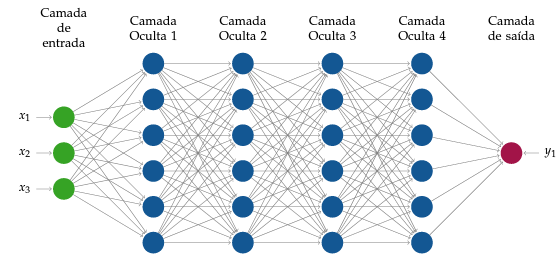
\includegraphics[scale=0.8]{imagens/arquitetura_redeneural.png}
    \subcaption*{Fonte: \cite{izbicki_mendonca2020}}
    \label{fig:arc_cpx_rnp}
    
\end{figure}

Note que as Figuras \ref{fig:arc_smp_rnp} e \ref{fig:arc_cpx_rnp} evidenciam um potencial muito grande de crescimento 
da rede e, naturalmente, esse aumento pode gerar um custo computacional elevado quando a rede estiver em treinamento.

\vspace{1cm}

\subsubsection{\textit{Forward propagation}}

O processo \textit{Forward propagation} (ou propagação direta) é o responsável por transmitir as informações,
 desde a camada de entrada, passando pelas camadas ocultas, até chegar na camada de saída. O \textit{Forward propagation}
  aplica a Equação \ref{neuronio} para cada neurônio presente nas camadas internas da rede neural. 
  Por isso temos, para cada j-ésimo neurônio, da camada $l$, a seguinte combinação linear:

\[
z_{j}^{(l)} = b_{j}^{(l)} + \sum_{i=1}^{d_{(l-1)}} w_{ij}a_{i}^{(l-1)} ,
\]

\noindent onde:
\begin{itemize}
    \item $w_{ij}$ é o peso associado à conexão entre o neurônio $i$ na camada $l-1$ e o neurônio $j$ na camada $l$;
    \item $a_{(i)}^{(l-1)}$ é a saída do neurônio i na camada anterior $(l-1)$;
    \item $b_{j}^{(l)}$ é o viés (bias) associado ao neurônio j na camada $l$.
\end{itemize}

Logo em seguida é aplicada uma função de ativação $g$ em $z_{j}^{(l)}$, sendo esta responsável por gerar o
 resultado final $a_{j}^{(l)}$, do o j-ésimo neurônio na l-ésima camada.

\[a_{i}^{(l)} = g(z_{i}^{(l)})\]

Esse processo vai ser realizado camada a camada, sequencialmente. Logo, considerando uma rede com H camadas
ocultas, o resultado da camada de saída $H+1$ é dado por:

\begin{equation}
    f(\textbf{x}) = \textbf{a}^{H+1} = g(b_{j}^{(H+1)} + \sum_{i=1}^{d_{H}} w_{ij}a_{i}^{H}).
\end{equation}


Note que a previsão da rede vem diretamente do resultado obtido da camada de saída, e esse depende da camada 
que o antecede e assim sucessivamente até chegar na camada de entrada.


\subsubsection{Função de perda}

Para otimizar o desempenho do modelo, é escolhida uma função de perda. Uma função bastante utilizada
para estimação de médias é a do erro do quadrático médio:

\[EQM(f) = \frac{1}{n} \sum_{k=1}^{n} (f(\textbf{x}_k) - y_k)^2\]

Essa função é uma indicadora do quão longe, em média, os valores preditos $f(x_k)$ estão distantes dos valores reais $y_k$. 
Note que o resultado da função $f$ depende exclusivamente dos parâmetros da rede (viés e pesos), por isso, 
a derivada da função de perda é 0, significa que  os parâmetros dessa rede minimizaram a perda. Entretanto,
 devido à complexidade desse modelo, é possível parar em pontos locais mínimos, que, dependendo do contexto, são
 suficiente ótimos. A Figura \ref{fig:pesos_lossfunc} ilustra esse comportamento:

\begin{figure}[H]
    \centering
    \caption{Comportamentos dos pesos em relação à função de perda. O ponto $w_A$ representa um ponto local mínimo e $w_B$ representa um ponto global mínimo.}
    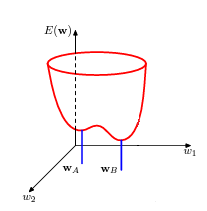
\includegraphics[scale=1]{imagens/pesos_loss_func.png}
    \caption*{Fonte: \cite{bishop2006pattern}}
    \label{fig:pesos_lossfunc}
    
\end{figure}

\subsubsection{\textit{Backpropagation}}

Como a função de perda $R(\theta)$ depende dos parâmetros (\textbf{$\theta$}) da rede, para se minimizar
 a função de perda, é necessário encontrar os valores de \textbf{$\theta$} que resolvam 
 esse problema de otimização. Para fazer isso, é necessário calcular o gradiente de  R(\textbf{$\theta$}) em 
 relação à \textbf{$\theta$} \cite{james2013introduction}, 

\begin{equation}
\nabla R(\theta) = \frac{\partial R(\theta)}{\partial \theta},     
\label{gradiente}
\end{equation}


A rede neural, durante todo o treinamento, aplica esse processo do cálculo do gradiente de R(\textbf{$\theta$}) 
em relação à \textbf{$\theta$}. Esse é um processo iterativo, que provoca alterações no valor de $\theta$ afim de 
conseguir minimizar a função de perda. Com isso a Equação \ref{gradiente} pode ser descrita nesse processo iterativo como:

\[
\nabla R(\theta^m) = \frac{\partial R(\theta)}{\partial \theta} \bigg\rvert_{\theta = \theta^m},
\]

\hspace{-1.5cm}onde $\theta = \theta^m$ significa que o cálculo do gradiente está sendo realizado na iteração $m$.

Para conseguir atualizar esse $\theta$, conforme é calculado o gradiente durante as iterações, é utilizada a técnica de gradiente descendente, que pode ser descrita como: 

\[
\theta^{m+1} \leftarrow \theta^{m} - \lambda\frac{\partial R(\theta^m)}{\partial \theta^m}
\]

\hspace{-1.5cm}sendo $\lambda$ o parâmetro que vai definir a magnitude de influência da derivada  $\frac{\partial R(\theta^m)}{\partial \theta^m}$ em $\theta^{m}$.

\begin{figure}[H]
    \centering
    \caption{Representação do método do gradiente descendente para a estimação de um parâmetro.}
    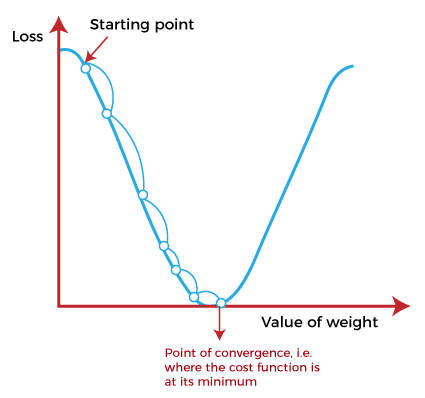
\includegraphics[scale=0.7]{imagens/gradient_descent.png}
    \caption*{Fonte: https://www.javatpoint.com/gradient-descent-in-machine-learning}
    \label{fig:gradient_descent}
    
\end{figure}

A Figura \ref{fig:gradient_descent} demonstra o processo do gradiente descendente. Os parâmetros são iniciados
 com algum valor e, conforme ocorre os processos iterativos de aprendizado, o parâmetro converge para um mínimo
  da função de perda. Note que a distância entre cada ponto é definida pelo $\lambda$ ou taxa de aprendizado.


Todo esse processo é realizado em cada parâmetro que existe na rede neural. Assim como as informações das variáveis
 são passadas camada a camada, iniciando na camada de entrada, passando pelas camadas ocultas e chegando na camada de 
 saída (\textit{Forward propagation}), a informação do resultado da rede na função de perda 
 é passada de forma contrária. Ou seja, o gradiente de cada parâmetro é calculado primeiro nas camadas mais próximas da saída,
  e essa informação é repassada para trás, chegando até os parâmetros da camada de entrada. Esse processo
   é chamado de \textit{Backpropagation} \cite{werbos1974beyond}.


\subsection{SHAP}

A estrutura de uma rede neural, por mais que proporcione bons resultados, mostra uma deficiência na parte interpretativa. 
Conhecida por ser uma "caixa-preta" pelo fato de sua estrutura ser muito complexa, existe a necessidade de se entender 
as predições feitas.
Para isso, existem técnicas que visam a interpretação de modelos de redes neurais, como por exemplo a
 técnica SHAP. Através dela é possível entender como as variáveis de entrada influenciam as previsões do modelo, 
 fornecendo explicações sobre sua lógica. Isso contribui para a 
 transparência, confiabilidade e aceitação dos modelos, além de auxiliar na detecção de viéses e discriminação. 

\subsubsection{Valores de Shapley}

Os valores de Shapley foram prpostos por Lloyd Shapley \cite{shapley1953value} no contexto da teoria de jogos, 
e essa técnica ganhou   força na área de inteligência artificial pela sua capacidade de conseguir interpretar modelos
 preditivos tidos como "caixa-preta". 
 
 No método criado por Shapley, havia uma quantidade de jogadores que exerciam
  juntos determinada atividade, e o intuito era observar o ganho que um jogador (ou um conjunto de jogadores), obtinha 
  ao ser adicionado para realizar a mesma tarefa, sem a presença do restante do grupo \cite{hart_1989}. 

Podemos definir \textbf{F} como o conjunto dos jogadores disponíveis para a realização da tarefa, 
logo $\textbf{F} = \{1,2,..., \textbf{M}\}$, onde \textbf{M} é o número total de jogadores.
Definindo \textbf{S} como uma coligação do conjunto \textbf{F} $(\textbf{S} \subseteq \textbf{F})$, temos, por exemplo, as seguintes possibilidades de \textbf{S}, quando \textbf{M} é igual a 3:

$$ \{\{\emptyset\},\{1\},\{2\},\{3\},\{1,2\},\{1,3\},\{2,3\},\{1,2,3\}\}$$

Existe também uma função que vai mapear um conjunto de valores e retornar um número real, chamada de $\nu$. Com isso, o retorno de $\nu(\textbf{S})$ é um número real que pode ser definido como 
o "trabalho da coligação \textbf{S}" ou o "trabalho dos jogadores presentes no conjunto \textbf{S}". Esse valor é equivalente ao total ganho que os jogadores podem obter caso trabalhem juntos em uma determinada coligação.

Para calcular o ganho ao adicionar $i$-ésimo jogador em uma tarefa, 
pode-se calcular o ganho quando é adicionado aquelo jogador na coligação menos o ganho da coligação sem 
a adição daquele jogador, ficando da seguinte maneira:

\begin{equation}
  \nu({\textbf{S} \cup \{i\})} - \nu({\textbf{S})}    
\end{equation}


No exemplo acima, para calcular o efeito da coligação \{3\}, pode-se realizar o seguinte processo:

\[
\text{Contribuição} \hspace{1mm} de \hspace{1mm} \{3\} = \nu(\{1,2,3\}) - \nu(\{1,2\})  
\]


Entretanto, considere que as variáveis (ou jogadores) \{2\} e \{3\} apresentam uma semelhança extraordinária.
 Ao calcular o ganho ao inserir \{2\} na coligação \{1,2\}, observamos um aumento substancial. No entanto,
  ao adicionar \{3\} à coligação \{1,2,3\}, o ganho é significativamente menor. Devido à semelhança no papel 
  desempenhado por essas variáveis, o maior ganho está vinculado à variável adicionada primeiro à coligação, 
  não necessariamente indicando que uma seja mais importante que a outra.

Por isso, para calcular o real ganho da variável \{i\}, é necessário testar todas as permutações de \textbf{F} 
(conjunto de jogadores) e obter a contribuição de \{i\} em cada uma delas, para então fazer a média dessas 
contribuições. Por exemplo, considerando 4 jogadores, \textbf{F} = \{1,2,3,4\}, suponha que estamos interessados em calcular
 a contribuição de \{3\}, logo, podemos obter a seguinte permutação de  \textbf{F}:

$$[3,1,2,4]$$

Calculando a contribuição de \{3\}, temos: 

$$\nu(\{3\}) - \nu(\emptyset) $$

Outra permutação poderia ser :

$$[2,4,3,1]$$

Calculando a contribuição de \{3\}, nessa permutação temos: 

$$\nu(\text{coligação} \hspace{1mm} de \hspace{1mm} [2,4,3]) - \nu(\text{coligação} \hspace{1mm} de \hspace{1mm} [2,4]) $$


É importante ressaltar que a função $\nu$ aceita a coligação como argumento, não a permutação. 
Uma coligação é um conjunto, onde a ordem dos elementos não tem importância, ao passo que uma permutação é uma 
coleção ordenada de elementos. Na permutação [3,1,2,4], por exemplo, 3 é a primeira variável adicionada, enquanto 
4 é a última. Portanto, para cada permutação, a ordem dos elementos pode influenciar na contribuição total, mas o
 ganho total da permutação depende apenas dos elementos, não da ordem. Assim:

\[\nu(\text{coligação} \hspace{1mm} de \hspace{1mm} [3,1,2,4]) = \nu(\{1,4,2,3\})\]

Sendo assim, para cada permutação \textbf{P}, é preciso primeiro calcular o ganho da coligação das variáveis que 
foram adicionadas antes de \{i\}, e esse conjunto pode ser chamado de coligação \textbf{S}. Feito isso, agora é 
preciso calcular o ganho das coligações que são formadas ao adicionar \{i\} em \textbf{S}, e podemos chamar
 isso de $\textbf{S} \cup \{i\}$. Com isso, a contribuição da variável \{i\}, denotada por $\phi_{i}$, é:

 Portanto, para cada permutação \textbf{P}, é necessário inicialmente calcular o ganho da coligação das variáveis
  que foram adicionadas antes de {i}, e esse conjunto pode ser referido como coligação \textbf{S}. Em seguida, é
   necessário calcular o ganho das coligações formadas ao adicionar {i} a \textbf{S}, e podemos representar isso 
   como $\textbf{S} \cup {i}$. Dessa forma, a contribuição da variável {i}, denotada por $\phi_{i}$, é:

\begin{equation}
 \phi_i = \frac{1}{|\textbf{F}|!}\sum_{\textbf{P}} [\nu(\textbf{S}\cup\{i\}) - \nu(\textbf{S})]
 \label{eq:value_shap_ini}
\end{equation}

O número total de permutações de \textbf{F} é $|\textbf{F}|!$. Logo, podemos dividir a soma das contribuições por $|\textbf{F}|!$ 
para encontrar o valor esperado de contribuição de \{i\}. A Figura \ref{fig:total_permuts_shap} mostra como é feito esse calculo
 para um determinado jogador $\{i\}$.

\begin{figure}[H]
    \centering
    \caption{Ganho do jogador 3 em relação a todas as permutações de jogadores.}
    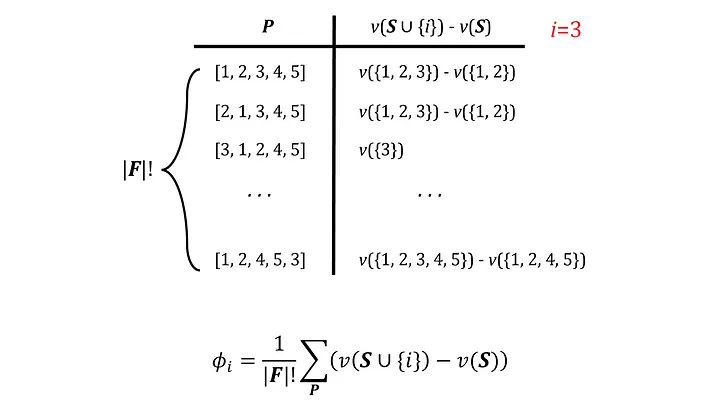
\includegraphics[scale=0.5]{imagens/shap.png}
    \caption*{Fonte: https://towardsdatascience.com/introduction-to-shap-values-and-their-application-in-machine-learning-8003718e6827}
    \label{fig:total_permuts_shap}
    
\end{figure}


É evidente que algumas permutações apresentam a mesma contribuição, contanto que suas coligações $\textbf{S}\cup{i}$ e \textbf{S}
 sejam idênticas. Para otimizar o cálculo da contribuição de cada permutação, é possível identificar quantas vezes a geração de
  permutações resultará em uma contribuição igual a outra.


Para fazer isso, é necessário descobrir quantas permutações podem ser formadas de cada coligação. Podemos definir
$\textbf{F} - \{i\}$ como o conjunto de todas as variáveis excluindo a variável \{i\}, e \textbf{S} como uma das
coligações de $\textbf{F} - \{i\} (\textbf{S} \subseteq  \textbf{F} - \{i\}$ ). 
Logo, para cada coligação \textbf{S} temos $|\textbf{S}|!$ possíveis permutações, que corresponde às possibilidades
de variáveis e suas respectivas ordens antes de adicionar a variável \{i\}.
Tendo os conjuntos $\textbf{S}\cup\{i\}$ e \textbf{S} definidos, resta agora achar as possíveis permutações
das variáveis restantes. E para saber o valor restante é preciso calcular o tamanho do conjunto gerado por:
\textbf{F} - ($\textbf{S}\cup\{i\}$ + 1)
que basicamente é o que resta das variáveis para completar o conjunto \textbf{F}.

 A Figura \ref{fig:permut_e_colig} ilustra o procedimento ao escolher o jogador $i=3$.
Na linha das coligações, são especificadas as possíveis coligações de \textbf{S}, que consistem nas
permutações dos jogadores 1 e 2, e a coligação $\{i\}$ cujo único elemento na coluna ${i}$, onde
o único elemento será o próprio $i$. Em seguida, são listadas as coligações dos jogadores restantes $\{4, 5\}$. 
Na linha das permutações, são apresentadas todas as permutações possíveis para \textbf{S}, $\{i\}$ e $\textbf{F}-\textbf{S}-\{i\}$. 
A última linha representa o tamanho do conjunto formado pela permutação/coligação descrita anteriormente.

\begin{figure}[H]
    \centering
    \caption{Relação entre permutações e coalisões.}
    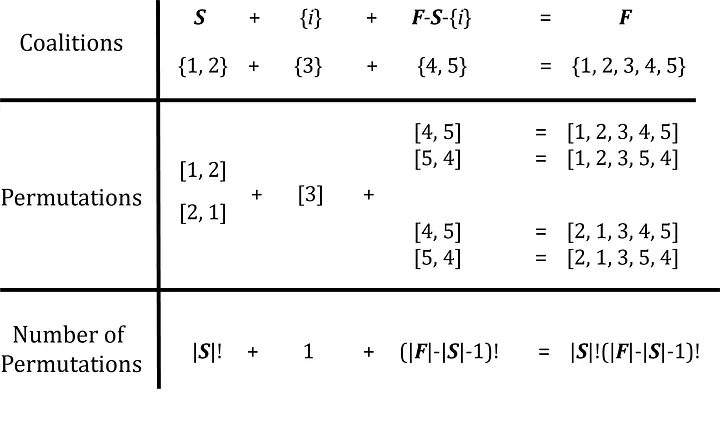
\includegraphics[scale=0.5]{imagens/shap1.png}
    \caption*{Fonte: https://towardsdatascience.com/introduction-to-shap-values-and-their-application-in-machine-learning-8003718e6827}
    \label{fig:permut_e_colig}
    
\end{figure}

Com isso, podemos reescrever a Equação \ref{eq:value_shap_ini} da seguinte maneira:

\[
\phi_i= 
\sum_{\textbf{S} \subseteq  \textbf{F} - \{i\}}
\frac{|\textbf{S}|!(|\textbf{F}| - |\textbf{S}| - 1)!}{|\textbf{F}|!}
[\nu(\textbf{S}\cup\{i\}) - \nu(\textbf{\textbf{S}})],
\]
\noindent\hspace{1.5cm} onde $\phi_i$ é o valor de shapley para a variável \{i\}.

\subsubsection{\textit{Shapley Additive Explanations}}

Fazendo o paralelo do valor de Shapley para o SHAP (\textit{Shapley Additive Explanations}), 
temos que os jogadores são as covariáveis do modelo e a função característica $\nu$ é equivalente à função $f(x)$
 responsável por fazer as predições.
 Assim, valores de SHAP são calculados para cada observação. Com isso, a fórmula do valor
  de SHAP, para cada a i-ésima covariável de determinada observação x é dada por:

\begin{equation}
\phi_i(f,\textbf{x})= 
\sum_{\textbf{S} \subseteq  \textbf{F} - \{i\}}
\frac{|\textbf{S}|!(|\textbf{F}| - |\textbf{S}| - 1)!}{|\textbf{F}|!}
[f_{\textbf{S}\cup\{i\}}(\textbf{x}_{\textbf{S}\cup\{i\}}) - f_{\textbf{S}}(\textbf{x}_{\textbf{S}})
]
\label{eq:SHAP}
\end{equation}

Perceba que $f_\textbf{S}(\textbf{x}_S)$ representa o resultado do modelo com somente as covariáveis
 que estão na coligação $\textbf{S}$, algo que na realidade não é permitido na maioria dos modelos. 
 Por isso, uma aproximação desse resultado é a seguinte:

\begin{equation}    
f_S(\textbf{x}_S) \approx E[f(\textbf{x}|\textbf{x}_S)] \approx 
\frac{1}{k} \sum_{i=1}^{k}
f(\textbf{x}_{\bar{S}}^{(i)}, \textbf{x}_S)
\label{eq:SHAP_detalhado}
\end{equation}

Ou seja, para $x_s$ fixo, toma-se variações do conjunto de variáveis que não pertencem ao conjunto $\textbf{x}_S$,
e calcula-se a média, conforme a Equação
\ref{eq:SHAP_detalhado}. Isso resulta na criação de uma
estimativa para $f(\textbf{x})$, levando em consideração apenas as variáveis presentes em $\textbf{S}$.
A Figura \ref{fig:calculo_esforço} ilustra o cálculo de 2, 3, 4, considerando $x = \{ x_1, x_2, x_3, x_4, x_5\}$,
$x_S = \{x_1, x_3, x_4\}$ e $x_{\bar{S}} = \{x_2, x_5\}$.


\begin{figure}[H]
    \centering
    \caption{Cálculo de $f_{\textbf{S}}$, sendo S o conjunto de variáveis $X_1, X_3, X_4$, dentre as observações de um conjunto de dados.}
    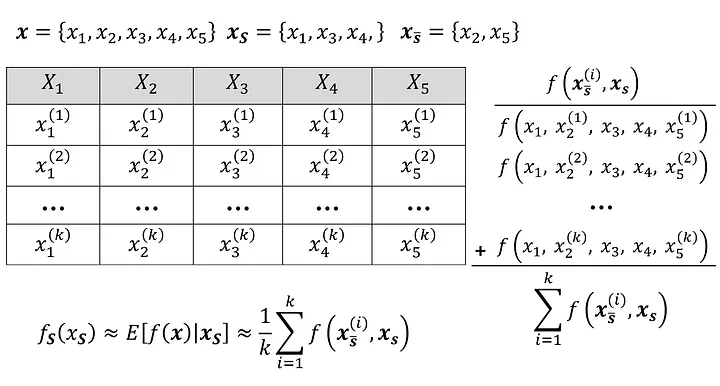
\includegraphics[scale=0.5]{imagens/shap_explicado.png}
    \caption*{Fonte: https://towardsdatascience.com/introduction-to-shap-values-and-their-application-in-machine-learning-8003718e6827}
    \label{fig:calculo_esforço}   
\end{figure}

Ao analisar a Figura \ref{fig:calculo_esforço}, tem-se que as covariáveis $X_1, X_3$ e $ X_4$ representam o conjunto $\textbf{S}$. 
Ao fixar $x_1, x_3$ e $ x_4$ dessas variáveis, respectivamente, é definido o conjunto $\textbf{x}_S$. 
Para obter $f_{\textbf{S}}(x_{\textbf{S}})$, que seria resultado do modelo somente com as covariáveis presentes 
em $\textbf{x}_S$, calcula-se $f$ para cada observação do conjunto de dados,
fixando $x_1, x_3$ e $ x_4$ na função e utilizando o valor das variáveis complementares, que neste caso são os
valores de $X_2$ e $X_5$, em suas respectivas observações. Feito isso, a média
desses valores é a estimativa
$f_{\textbf{S}}(x_{\textbf{S}})$.

Com $f_{\textbf{S}}(x_{\textbf{S}})$ estimado, é possível calcular a Equação \ref{eq:SHAP}. Os dados que a técnica SHAP 
utiliza são divididos em 2 tipos: as observações necessárias para a estimação de $f_{\textbf{S}}(x_{\textbf{S}})$
e as observações em que se deseja calcular o valor de SHAP. 



A avaliação do desempenho dos modelos é fundamental para mensurar sua eficácia nas predições ou classificações. 
A utilização de estratégias que resumem o desempenho por meio de métricas específicas é crucial nesse processo.
A análise dessas métricas proporciona uma compreensão mais aprofundada do modelo, permitindo identificar pontos 
fortes e áreas de melhoria. Essa avaliação não apenas valida a qualidade das previsões, mas também orienta os próximos
passos na pesquisa, direcionando ajustes necessários no modelo ou indicando caminhos para refinamento. 
Dessa forma, a escolha e interpretação adequadas das métricas são passos essenciais para uma avaliação informada 
e um progresso significativo na pesquisa \cite{geron2019hands}.

\subsubsection{Matriz de confusão}

A matriz de confusão é uma tabela usada para avaliar o desempenho de um modelo de classificação.
Seu papel é de expor os resultados das predições do modelo quando comparadas com os valores reais.

A matriz de confusão organiza as previsões do modelo em quatro categorias, comumente chamadas de Verdadeiro Positivo (VP), 
Falso Positivo (FP), Verdadeiro Negativo (VN) e Falso Negativo (FN). Essas categorias são definidas da seguinte maneira:

\begin{itemize}
  \item Verdadeiro Positivo (VP): Exemplos que foram corretamente classificadas como pertencentes à classe positiva.
  \item Falso Positivo (FP): Exemplos que foram erroneamente classificadas como pertencentes à classe positiva, quando na verdade pertencem à classe negativa.
  \item Verdadeiro Negativo (VN): Exemplos que foram corretamente classificadas como pertencentes à classe negativa. 
  \item Falso Negativo (FN): Exemplos que foram erroneamente classificadas como pertencentes à classe negativa, quando na verdade pertencem à classe positiva.
\end{itemize}

\begin{table}[h]
  \centering
  \begin{tabular}{cc|cc|}
    \cline{3-4}
  & & \multicolumn{2}{c|}{\textbf{Previsão}} \\ \cline{3-4}
  & & \textbf{Negativo} & \textbf{Positivo} \\ \hline
  \multicolumn{1}{|c|}{\multirow{2}{*}{\textbf{Real}}} & \textbf{Negativo} & Verdadeiro Negativo (VN) & Falso Positivo (FP) \\  
  \multicolumn{1}{|c|}{} & \textbf{Positivo} & Falso Negativo (FN) & Verdadeiro Positivo (VP) \\ \hline
  \end{tabular}
  \caption{Matriz de confusão}
  \label{table:confusion_matrix}
\end{table}

\subsubsection{Acurácia}
A acurácia é a proporção de predições corretas feitas por um modelo em relação ao número total de predições. 
A fórmula básica para calcular a acurácia é dada por:

\begin{equation}
  \text{Acurácia} = \frac{\text{Número de predições corretas}}{\text{Número total de predições}} = \frac{VP+VN}{VP+VN+FP+FN}
\end{equation}

Essa métrica fornece uma visão geral do desempenho do modelo, indicando a porcentagem de instâncias corretamente classificadas.
No entanto, a acurácia pode ser uma medida inacurada em casos onde as classes não estão balanceadas. 
Em situações desse tipo, um modelo que prevê sempre a classe majoritária pode ter uma acurácia alta, mesmo que não seja eficaz.

\subsubsection{Precisão}

A precisão é definida como a proporção de exemplos classificados corretamente como positivos, em 
relação ao total de exemplos classificados como positivos (verdadeiros positivos mais falsos positivos).

\begin{equation}
  \text{Precisão} = \frac{VP}{VP + FP}
\end{equation}

A precisão é particularmente útil quando os falsos positivos são mais problemáticos ou custosos
em comparação com os falsos negativos. Por exemplo, em um sistema de detecção de spam, classificar 
erroneamente um e-mail legítimo como spam (falso positivo) pode ser mais prejudicial do que deixar
passar um e-mail de spam (falso negativo).

\subsubsection{Recall}

O recall, também conhecido como sensibilidade, é outra métrica utilizada no contexto de classificação, 
focada em capturar a proporção de exemplos positivos que foram corretamente identificados pelo modelo,
em relação ao total de exemplos positivos existentes.

\begin{equation}
  \text{Recall} = \frac{VP}{VP + FN}
\end{equation}

O recall é especialmente útil quando os falsos negativos (exemplos positivos não identificadas pelo modelo) 
são mais críticos ou custosos do que os falsos positivos. Por exemplo, em um sistema de detecção de fraudes,
é crucial identificar todas as transações fraudulentas, mesmo que isso signifique aceitar algumas transações 
normais erroneamente classificadas como fraudulentas.


\subsubsection{F1-score}

O F1-score é uma métrica de avaliação que combina as métricas de precisão e recall em um único valor. 

\begin{equation}
  F1 = 2 \cdot \frac{\text{Precisão} \cdot \text{Recall}}{\text{Precisão} + \text{Recall}}
\end{equation}

O F1-score é a média harmônica entre a precisão e o recall. A média harmônica é utilizada porque penaliza extremos, 
sendo particularmente sensível a baixos valores em qualquer uma das métricas.

O F1-score varia de 0 a 1, onde 1 indica o melhor desempenho possível, equilibrando tanto a precisão quanto o recall.
Essa métrica é particularmente útil quando há um desequilíbrio significativo entre as classes, 
pois é menos sensível a grandes quantidades de verdadeiros negativos.